%
% File acl2018.tex
%
%% Based on the style files for ACL-2017, with some changes, which were, in turn,
%% Based on the style files for ACL-2015, with some improvements
%%  taken from the NAACL-2016 style
%% Based on the style files for ACL-2014, which were, in turn,
%% based on ACL-2013, ACL-2012, ACL-2011, ACL-2010, ACL-IJCNLP-2009,
%% EACL-2009, IJCNLP-2008...
%% Based on the style files for EACL 2006 by 
%%e.agirre@ehu.es or Sergi.Balari@uab.es
%% and that of ACL 08 by Joakim Nivre and Noah Smith

%\documentclass[11pt,a4paper]{article}
%\usepackage{hyperref}
%\usepackage[hyperref]{acl2018}
%\usepackage{times}
%\usepackage{latexsym}
%\usepackage{ifthen}
%\usepackage{url}
%\usepackage{amsmath}
%\usepackage{amsthm}
%\usepackage{amsfonts}
%\usepackage{amssymb}
%\usepackage{bbm}
%\usepackage{graphicx}
%\usepackage{subcaption}
%\usepackage{booktabs}
%\usepackage{soul}
%
%%% Steve's stuff
%\usepackage{color}
%\usepackage{colortbl}
%\usepackage{algorithm}
%\usepackage{algorithmic}
%\usepackage{amsthm}

%    \newtheorem{lemma}{Lemma}[section]
%    \newtheorem{proposition}{Proposition}[section]
%    \newtheorem{theorem}{Theorem}[section]
%    
%    \newtheoremstyle{TheoremNum}
%        {\topsep}{\topsep}              %%% space between body and thm
%        {\itshape}                      %%% Thm body font
%        {}                              %%% Indent amount (empty = no indent)
%        {\bfseries}                     %%% Thm head font
%        {.}                             %%% Punctuation after thm head
%        { }                             %%% Space after thm head
%        {\thmname{#1}\thmnote{ \bfseries #3}}%%% Thm head spec
%    \theoremstyle{TheoremNum}
%    \newtheorem{thm}{Theorem}
%    \newtheorem{corl}{Corollary}
%    \newtheorem{lem}{Lemma}
%    \newtheorem{prop}{Proposition}
    
\chapter{\label{chap:price} The price of debiasing automatic metrics in natural language evaluation}
\providecommand{\muh}{\hat{\mu}}
\providecommand{\yh}{\hat{y}}


In natural language tasks such as knowledge base population, text summarization or open-response question answering, a significant challenge is simply evaluating the performance of automated systems because of the large diversity of possible outputs.
% ^^ Include the fact that the domain has shifted?
Existing fully-automatic methods for evaluating these systems rely on an \textit{incomplete} set of annotated references which lead to \textit{systematic biases} against certain system improvements: in other words, genuinely good ideas are systematically discarded simply because of limitations in our evaluation methodology.
As a result, human evaluation, which can be prohibitively expensive, has remained the most trusted mode of evaluation for these tasks.
In this work, we show how one can decrease the costs of incorporating human feedback through the design of appropriate statistical estimators. 
% JARGON: contrast between tasks which are very straightforwards.
%
% Some tasks are very clear cut: classification, parsing, question answering.
% others we really don't know what we're doing.

First, we consider the \textit{``finite incompleteness''} setting where the output space is too large to exhaustively annotate, but we may still expect significant overlap between the output of different systems. 
Naively combining annotations from different systems leads to a representation bias.
Here, we show that the cost of obtaining human feedback can be significantly amortized by using a novel importance-reweighted estimator.  
We apply this estimator to design a new evaluation methodology for knowledge base population and empirically show that the cost of evaluating precision and recall within this framework can be reduced by a factor of 4.

Next, we consider the \textit{``infinite incompleteness''} setting wherein few, if any, systems ever produce identical output.
Traditionally, the community has relied on similarity-based automatic metrics such as BLEU or ROUGE to compare the outputs produced by different systems.
Unfortunately, these metrics have been shown to correlate poorly with human judgment and thus introduce bias in evaluation.
We derive an unbiased estimator that optimally combines these automatic metrics with human feedback.
Our theoretical results allow us to characterize potential cost reductions only in terms of the tasks' subjectivity, measured by inter-annotator variance, and the automatic metrics' quality, measured by correlation with human judgments.
On two popular natural language generation tasks, question answering and summarization, we empirically show that currently we can achieve at most a 7--13\% reduction in cost on two tasks, exposing fundamental limitations in \hyphenation{de-biasing} current automatic metrics.

Finally, we turn our attention to \textit{incompleteness in the training data}, particularly in low-resource settings.
Here, our machine learning systems simply have not seen sufficient training data for a particular phenomenon to accurately make predictions for them at test time. 
To tackle this incarnation of incompleteness, we train a system ``on-the-job'' by requesting for human feedback in real-time while the model is deployed to economically fill in holes in the training data and thus resolve uncertainty in the model.
Our key idea here is to cast the problem as a stochastic game based on Bayesian decision theory, which allows us to balance latency, cost, and accuracy objectives in a principled way.
When tested on three classification tasks---named-entity recognition, sentiment classification, and image classification---we obtain an order of magnitude reduction in cost compared to full human annotation even when starting from zero training examples, while also boosting performance relative to a classical supervised model on the expert-provided labels.


\section{Introduction}
\label{sec:intro}

\begin{figure}[t]
  \centering
  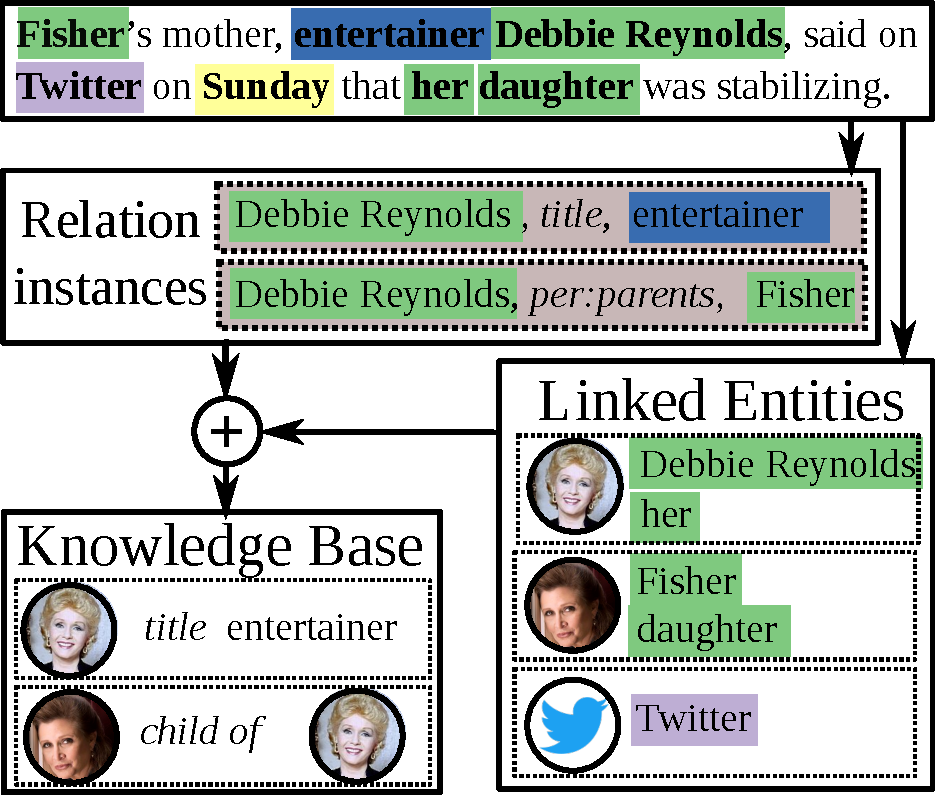
\includegraphics[width=0.6\columnwidth]{figures/entities-example.pdf}
  \caption[Example: KBP]{\label{fig:example} An example describing entities and relations in knowledge base population.}
\end{figure}

% (1 page w/ figure)
% Goal: remind the reader what information extraction is, what its relation to knowledge base population is and why it is important. Hook question.
Harnessing the wealth of information present in unstructured text online has been a long standing goal for the natural language processing community.
In particular, knowledge base population seeks to automatically construct a knowledge base consisting of relations between entities from a document corpus. % (\reffig{example}).
Knowledge bases have found many applications including question answering \citep{berant2013freebase, fader2014open,reddy2014large}, automated reasoning \citep{kalyanpur2012structured} and dialogue~\citep{han2015exploiting}.

% Evaluation @ scale poses problem. -- pooling methodology
Evaluating these systems remains a challenge as it is not economically feasible to exhaustively annotate every possible candidate relation from a sufficiently large corpus.
As a result, a pooling-based methodology is used in practice to construct datasets, similar to them methodology used in information retrieval \citep{sparck1975report, harman1993trec}.
For instance, at the annual NIST TAC KBP evaluation, all relations predicted by participating systems are pooled together, annotated and released as a dataset for researchers to develop and evaluate their systems on.
However, during development, if a new system predicts a previously unseen relation it is considered to be wrong even if it is correct.
The discrepancy between a system's true score and the score on the pooled dataset is called \emph{pooling bias} and is typically assumed to be insignificant in practice~\citep{zobel1998reliable}.

% Key finding: pooling bias
The key finding of this paper contradicts this assumption and shows that the pooling bias is actually significant, and it penalizes newly developed systems by 2\% \fone{} on average (\refsec{kbpo:analysis}).
Novel improvements, which typically increase scores by less than 1\% \fone{} on existing datasets, are therefore likely to be clouded by pooling bias during development.
Worse, the bias is larger for a system which predicts qualitatively different relations systematically missing from the pool.
% anti-solution
Of course, systems participating in the TAC KBP evaluation do not suffer from pooling bias, but this requires researchers to wait a year to get credible feedback on new ideas.
% TODO: I would like to add something about how ML methods are hosed, but perhaps for later?
% Chris's comment:  - Not addressed by Zobel, but I feel there is a big difference between whether this bias is a problem when used just for evaluation or also for system training (machine learning). If just for evaluation, some bias is a shame but doesn’t really badly effect things. If you are training systems assuming that your result set is the complete set of positives, then I feel that the effect of this bias is much more harmful, and this is the part that really impedes progress.

This bias is particularly counterproductive for machine learning methods as they are trained assuming the pool is the complete set of positives.
Predicting unseen relations and learning novel patterns is penalized.
The net effect is that researchers are discouraged from developing innovative approaches, in particular from applying machine learning, thereby slowing progress on the task. 

%These observations may explain why rule-based systems still play such a significant role in the top submissions at TAC KBP, and why, even after 8 years, top automated systems achieve scores of only about 35\% \fone{} while human annotators score above 60\% \fone{} on the same task.

% Solution: on-demand evaluation.
Our second contribution, described in \refsec{method}, addresses this bias through a new evaluation methodology, \emph{on-demand evaluation},
which avoids pooling bias by querying crowdworkers,
while minimizing cost by leveraging previous systems' predictions when possible.
%When a researcher submits a new system's predictions to our evaluation platform,
%we carefully sample a subset of its predictions and have crowdworkers judge them.
%just enough of its predictions to guarantee an accurate estimate of scores and have crowdworkers judge them.
We then compute the new system's score based on the predictions of past systems using importance weighting.
As more systems are evaluated, the marginal cost of evaluating a new system decreases.
% Experimental results.
We show how the on-demand evaluation methodology can be applied to knowledge base population in \refsec{application}.
Through a simulated experiment on evaluation data released through the TAC KBP 2015 Slot Validation track, we show that we are able to obtain unbiased estimates of a new systems score's while significantly reducing variance.

Finally, our third contribution is an implementation of our framework as a publicly available evaluation service at \url{https://kbpo.stanford.edu}, where researchers can have their own KBP systems evaluated.
The data collected through the evaluation process could even be valuable for relation extraction, entity linking and coreference, and will also be made publicly available through the website.
We evaluate three systems on the 2016 TAC KBP corpus for about \$150 each (a fraction of the cost of official evaluation).
We believe the public availability of this service will speed the pace of progress in developing KBP systems.

% NOTE: Figure is here because LaTeX refuses to place is with section 2 on its own.
\begin{figure}[t]
  \begin{subfigure}{0.49\textwidth}
    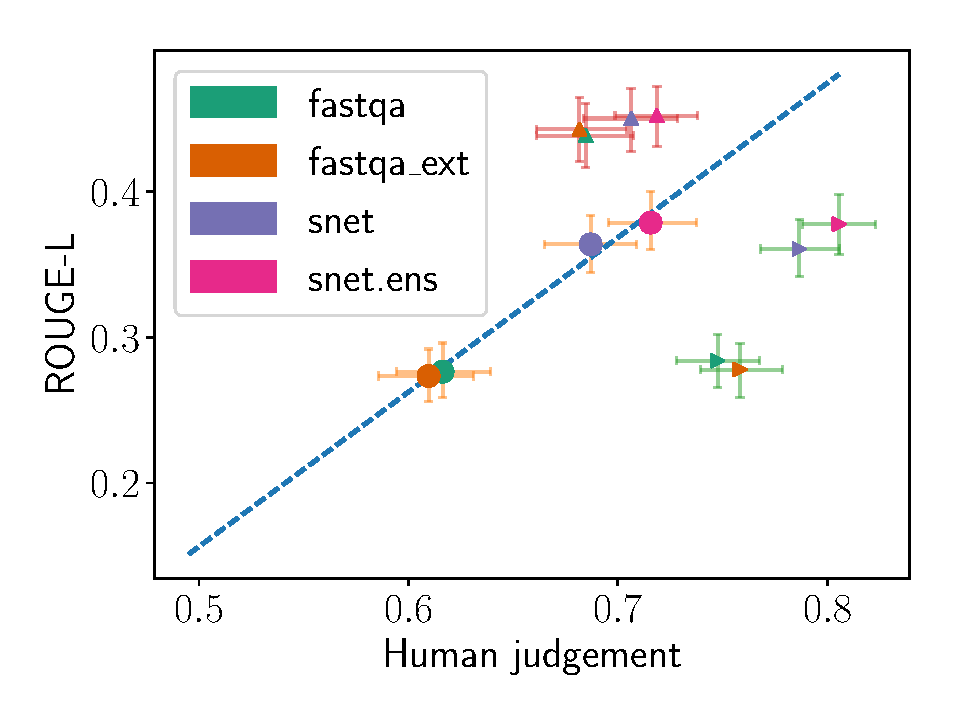
\includegraphics[width=\textwidth]{figures/msmarco_bias}
    \caption{\label{fig:bias-msmarco-system} System-level correlation on the MS MARCO task}
  \end{subfigure}
  \hfill
  \begin{subfigure}{0.49\textwidth}
    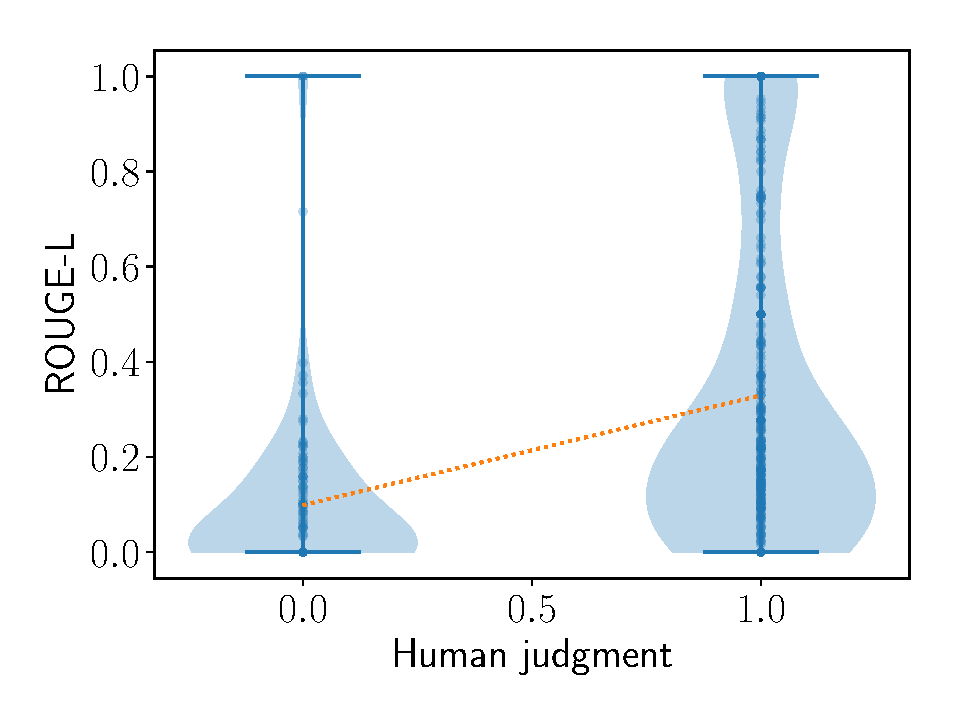
\includegraphics[width=\textwidth]{figures/msmarco_instance_correlation}
    \caption{\label{fig:bias-msmarco-instance} Instance-level correlation for the \texttt{fastqa} system}
  \end{subfigure}
  \caption[System-level vs instance-level correlation on MS MARCO]{\label{fig:bias-msmarco}
  %We compare system-level and instance-level correlations between the ROUGE-L automatic metric and some human metric.
  (a) At a system-level, automatic metrics (ROUGE-L) and human judgment correlate well, but (b) the instance-level correlation plot
  (where each point is a system prediction) shows that the instance-level correlation is quite low ($\rho = 0.31$).
  %The instance-level correlation plot (where each point is an example) reveals that there is a large proportion of good answers that scored poorly by ROUGE, effectively ``hiding'' them from evaluation.
  As a consequence, if we try to locally improve systems to produce better answers ($\triangleright$ in (a)),
  they do not significantly improve ROUGE scores and vice versa ($\vartriangle$).
  %\pl{can we get rid of the left arrows to simplify / save space?}
  %At the same time, system changes that hurt human evaluation scores are not reflected by the automatic metric either (left arrows).
  %\ac{I don't know how to properly reference the fact that circles are systems and.} 
  }
\end{figure}


\section{\label{sec:bias} Bias in automatic evaluation}

% What does bias mean in natural language evaluation.
%The central theme of this paper is to bring to the fore a discussion of how we evaluate our generation systems.
%It is well understood that current automatic metrics are poorly correlated with human judgment at the instance-level~\citep{},
%yet, somewhat surprisingly they can still have high \textit{system-level} correlations~\citep{novikova2017why}.
%Does this imply that we should be able to assess system improvements?
%We will argue that high system-level correlations are insufficient.
%\ac{should I cite original ROUGE papers as basically indicating high system level correlations}
% PL: sure, but maybe not essential
% TODO: Change to a "as a result" using novikova results!

%use the automatic metric to compare systems and thus make incremental progress towards a better system.
%Is this the complete story?

%\begin{table*}
%  \input{examples.table}
%  \caption{\label{tab:examples} Examples on MS MARCO where the proposed answer is correct, but ROUGE-L is low
%  due to multiple correct answers.}
%\end{table*}

\begin{table}[!p]
  \centering
  \input{examples-1.table}
  \caption[Examples highlighting where automatic metric and human judgments agree or disagree on MS MARCO.]{\label{tab:examples-msmarco}
    Examples highlighting the different modes in which the automatic metric and human judgments may agree or disagree on the MS MARCO task.
    Human annotators rated answer correctness (\texttt{AnyCorrect}) and the automatic metric used is ROUGE-L (higher is better).
    A majority of responses from systems were actually correct but poorly scored according to ROUGE-L.
  }
\end{table}

\begin{table}[!p]
  \centering
  \input{examples-2.table}
  \caption[Examples highlighting where automatic metric and human judgments agree or disagree on CNN/Daily Mail.]{\label{tab:examples-cdm}
    Examples highlighting the different modes in which the automatic metric and human judgments may agree or disagree on the CNN/Daily Mail task.
    Human judgment scores used are post-edit distance (\texttt{Edit}) (lower is better) and the automatic metric used is sentence vector similarity with the reference (higher is better).
    A significant number of examples which are scored highly by VecSim are poorly rated by humans, and likewise many examples scored poorly by VecSim are highly rated by humans.
  }
\end{table}

It is well understood that current automatic metrics tend to correlate poorly with human judgment at the instance-level.
% Example 1: novikova 
For example, \citet{novikova2017why} report correlations less than $0.3$ for a large suite of word-based and grammar-based evaluation methods on a generation task.
% Example 2: Liu
Similarly, \citet{liu2016evaluate} find correlations less than $0.35$ for automatic metrics on a dialog generation task in one domain, but find correlations with the same metric dropped significantly to less than $0.16$ when used in another domain. 
Still, somewhat surprisingly, several automatic metrics have been found to have high \textit{system-level} correlations~\citep{novikova2017why}.
What, then, are the implications of having a low instance-level correlation?  

As a case study, consider the task of open-response question answering:
  here, a system receives a human-generated question and must \textit{generate} an answer from some given context, e.g.\ a document or several webpages.
  We collected the responses of several systems on the MS MARCOv1 dataset~\citep{nguyen2016ms} and crowdsourced human evaluations of the system output
  (see \refsec{tasks} for details).
%ROUGE-L and human judgment appear to be well correlated at the system-level (\reffig{bias-msmarco-system}) \stm{isn't this a bs claim since we really only have two systems? depend on references?},
%is high\footnote{%
  %The correlation measured between systems in \reffig{bias-system-msmarco} is $\rho = 0.99$, the correlation is computed with two pairs of similar systems and hence this correlation is not a fair estimate.} 

The instance-level correlation (\reffig{bias-msmarco-instance}) is only $\rho = 0.31$.
A closer look at the instance-level correlation reveals that
while ROUGE is able to correctly assign low scores to bad examples (lower left),
it is bad at judging good examples and often assigns them low ROUGE scores (lower right)---see \reftab{examples} for examples.
This observation agrees with a finding reported in \citet{novikova2017why} that automatic metrics correlate better with human judgments on bad examples than average or good examples. 

% PL: breaks the flow, so cut
%This observation was also made by \citet{novikova2017why} in the context of evaluating dialogue generation.
%Though variants of automatic metrics such as METEOR~\citep{lavie2009meteor} were designed
%to better capture linguistic variation they still have low correlation.

% Improve ROUGE, no human quality; improve human quality
Thus, as \reffig{bias-msmarco}(a) shows, we can improve low-scoring ROUGE examples without improving their human judgment ($\vartriangle$) and vice versa ($\triangleright$).
Indeed, \citet{conroy2008mind} report that summarization systems were optimized for ROUGE during the DUC challenge~\citep{dang2006overview}
until they were indistinguishable from the ROUGE scores of human-generated summaries, but the systems had hardly improved on human evaluation.
% PL: save space % we're under now and I think this is an important point
Hill-climbing on ROUGE can also lead to a system that does worse on human scores, e.g.\ in machine translation~\citep{wu2016google}.
Conversely, genuine quality improvements might not be reflected in improvements in ROUGE\@.
This bias also appears in pool-based evaluation for knowledge base population \citep{chaganty2017unbiased}.
Thus the problems with automatic metrics clearly motivate the need for human evaluation,
but can we still use the automatic metrics somehow to save costs?

% PL: I like this, but I think we don't have space to explain it properly
%These are interesting examples that we would like our systems to be able to handle,
%but because automatic metrics correlate so poorly on this subset, they are in effect ``hidden'' from our evaluation.
%To demonstrate this point, we took each system in our earlier experiment and swapped any output that is scored poorly by ROUGE with that of another system
%to do either better (left arrow) or worse (right arrow) than the original output as evaluated by humans.
%The ROUGE scores of the perturbed systems remain the same while the human evaluation scores are significantly affected.
%On the other hand, if we perturbed the input to only improve the ROUGE scores of examples which scored poorly on ROUGE scores (up arrow),
%we see essentially no improvements in human judgment scores.
%they found that as systems tuned using ROUGE they successively improved on the automatic metric until they were indistinguishable from human performance while still hardly budging on human evaluations.

% Conclusion:
%   - simply having high system-level correlations is insufficient for a metric.
%   - instead, we should strive to meet human judgment and be unbiased statistically.
%The ramifications of this are that if we were to make a genuine improvement in a system
%that happens to improve upon difficult examples (i.e.\ move more output to the lower right corner),
%we would not observe any improvement in ROUGE and are likely not to pursue such a direction further.\@
%Indeed, \citet{conroy2008mind} report that as summarization systems tuned using the ROUGE metric for the DUC challenge~\citet{},
%they successively improved on the automatic metric until they were indistinguishable from human ROUGE scores while hardly budging on human evaluations.

%\stm{The points made in the next couple sentences are pretty weak and vague. You mention much more convincing points in the Related Work. Can you put some of those here?}
%This gap between improving automatic metric scores and human evaluation scores was also observed by  when comparing the performance of summarization systems in the DUC summarization challenges~\citep{} across years.
%In fact there is already bias: systems that exist in the literature
%are likely to have high human-automatic correlation since that's how they have been developed.
%\pl{not sure if this solid}
% PL: wanted to talk about genuine improvements

%\ac{I don't know how to end this section yet. I want it to lead into our approach of being unbiased.}

%Thus, we should care not about finding automatic metrics that have high
%system-level correlations with human judgments, but rather ways of actually
%measuring human judgment better.
%\pl{a bit too preachy}
%This is what we mean by unbiased!

% - Statistically, it's not equal to what we posit.
% - Practically, it means that the evaluation systematically favors one set of systems over another.
% - Understandable when system-level correlation is low, but should high system-level correlations simply be the goal of evaluation metrics?
% - We argue not.

\section{On-demand evaluation with importance sampling}
\label{sec:method}

Pooling bias is fundamentally a sampling bias problem where relation instances from new systems are underrepresented in the evaluation dataset.
We could of course sidestep the problem by exhaustively annotating the entire document corpus, by annotating all mentions of entities and checking relations between all pairs of mentions. However, that would be a laborious and prohibitively expensive task:
using the interfaces we've developed (\refsec{evaluation}), it costs about \$15 to annotate a single document by non-expert crowdworkers, resulting in an estimated cost of at least \$1,350,000 for a reasonably large corpus of 90,000 documents \citep{dang2016kbp}.
The annotation effort would cost significantly more with expert annotators.
% TODO: highlight contrast with pooling.
In contrast, \textit{labeling} 
%\pl{be consistent with terminology: labeling?} 
relation instances from system predictions
can be an order of magnitude cheaper than finding them in documents: using our interfaces, it costs only about \$0.18 to verify each relation instance compared to \$1.60 per instance extracted through exhaustive annotations.
%\pl{why the diff between 0.18 and 1.60?  Isn't it the same problem of labeling an instance?}

We propose a new paradigm called on-demand evaluation which takes a lazy approach to dataset construction by annotating predictions from systems \textit{only when they are underrepresented}, thus correcting for pooling bias as it arises.
In this section, we'll formalize the problem solved by on-demand evaluation independent of KBP and describe a cost-effective solution that allows us to accurately estimate evaluation scores
%metrics \pl{be consistent: scores} 
without bias using importance sampling.
We'll then instantiate the framework for KBP in \refsec{application}.

\subsection{Problem statement}
Let $\sX$ be the universe of %candidate predictions (e.g.\, relation instances),
(relation) instances,
  $\sY \subseteq \sX$ be the unknown subset of correct instances,
  $X_1, \ldots X_m \subseteq \sX$ be the predictions for $m$ systems,
  and let $Y_i = X_i \cap \sY$.
Let $X = \Union_{i=1}^m X_i$ and $Y = \Union_{i=1}^m Y_i$.
Let $f(x) \eqdef \I[x \in \sY]$ and $g_i(x) = \I[x \in X_i]$, then the precision, $\pi_i$, and recall, $\recall_i$, of the set of predictions $X_i$ is
\begin{align*}
  %\pi_i  &\eqdef \E_{x \sim X_i}[f(x)] &
  %\recall_i &\eqdef \E_{x \sim \sY}[g_i(x)],
  \pi_i  &\eqdef \E_{x \sim p_i}[f(x)] &
  \recall_i &\eqdef \E_{x \sim p_0}[g_i(x)],
\end{align*}
where $p_i$ is a distribution over $X_i$ and $p_0$ is a distribution over $\sY$.
We assume that $p_i$ is known, e.g.\, the uniform distribution over $X_i$
and that we know $p_0$ up to normalization constant and can sample from it.

In on-demand evaluation, we can query $f(x)$ (e.g.\, labeling an instance) or draw a sample from $p_0$;
typically, querying $f(x)$ is significantly cheaper than sampling from $p_0$.
We obtain prediction sets $X_1, \ldots, X_m$ sequentially as the systems are submitted for evaluation.
Our goal is to estimate $\pi_i$ and $\recall_i$ for each system $i = 1, \dots, m$.

\subsection{Simple estimators}
We can estimate each $\pi_i$ and $\recall_i$ independently with simple Monte Carlo integration. % from $p_i$ and $p_0$ respectively.
Let $\Xh_1, \ldots, \Xh_m$ be multi-sets of $n_1, \ldots, n_j$ i.i.d.~samples from $X_1, \ldots, X_m$ respectively, and let $\Yh_0$ be a multi-set of $n_0$ samples drawn from $\sY$.
Then, the simple estimators for precision and recall are:
\begin{align*}
  \pih_i^{\text{(simple)}} &= \frac1{n_i}\! \sum_{x \in \Xh_i}\! f(x) & \recallh_i^{\text{(simple)}} &= \frac1{n_0}\! \sum_{x \in \Yh_0}\! g_i(x).
\end{align*}

\subsection{Joint estimators\footnote{Proofs for claims made in this section can be found in \refapp{sampling} of the supplementary material.}}
\label{sec:joint}
The simple estimators are unbiased but have wastefully large variance
because evaluating a new system does not leverage labels acquired for previous
systems.  %\paragraph{Estimation Algorithm}

On-demand evaluation with the joint estimator works as follows:
First $\Yh_0$ is randomly sampled from $\sY$ once when the evaluation framework is launched.
For every new set of predictions $X_m$ submitted for evaluation, the minimum number of samples $n_m$ required to accurately evaluate $X_m$ is calculated based on the current evaluation data, $\Yh_0$ and $\Xh_1, \ldots, \Xh_{m-1}$.
Then, the set $\Xh_m$ is added to the evaluation data by evaluating $f(x)$ on $n_m$ samples drawn from $X_m$.
Finally, estimates $\pi_i$ and $\recall_i$ are updated for each system $i = 1,\ldots,m$ using the joint estimators that will be defined next.
%requires us to spend money to collect data for every new system submitted.
In the rest of this section, we will answer the following three questions:
\begin{enumerate}
    \itemsep0pt
  \item How can we use all the samples $\Xh_1, \ldots \Xh_m$ when estimating the precision $\pi_i$ of system $i$?
  \item How can we use all the samples $\Xh_1, \ldots, \Xh_m$ with $\Yh_0$ when estimating recall $\recall_i$?
  \item Finally, to form $\Xh_m$, how many samples should we draw from $X_m$ given existing samples and $\Xh_1, \ldots, \Xh_{m-1}$ and $\Yh_0$?
\end{enumerate}

\paragraph{Estimating precision jointly.}
Intuitively, if two systems have very similar predictions $X_i$ and $X_j$, we should be able to use samples from one to estimate precision on the other.
However, it might also be the case that $X_i$ and $X_j$ only overlap on a small region, in which case the samples from $X_j$ do not accurately represent instances in $X_i$ and could lead to a biased estimate.
We address this problem by using importance sampling \citep{owen2013monte}, a standard statistical technique for estimating properties of one distribution using samples from another distribution.

In importance sampling, if $\Xh_i$ is sampled from $q_i$, then $\frac{1}{n_i} \sum_{x \in \Xh_i} \frac{p_i(x)}{q_i(x)} f(x)$ is an unbiased estimate of $\pi_i$.
We would like the proposal distribution $q_i$ to both leverage samples from all $m$ systems and be tailored towards system $i$.
To this end, we first define a distribution over systems $j$, represented by probabilities $w_{ij}$.
Then, define $q_i$ as sampling a $j$ and drawing $x \sim p_j$;
formally $q_i(x) = \sum_{j=1}^m w_{ij} p_j(x)$.

We note that $q_i(x)$ not only significantly differs between systems, but also changes as new systems are added to the evaluation pool.
Unfortunately, the standard importance sampling procedure requires us to draw and use samples from each distribution $q_i(x)$ independently and thus can not effectively reuse samples drawn from different distributions.
To this end, we introduce a practical refinement to the importance sampling procedure:
we independently draw $n_j$ samples according to $p_j(x)$ from each of the $m$ systems independently 
and then numerically integrate over these samples using the weights $w_{ij}$ to ``mix'' them appropriately to produce and unbiased estimate of $\pi_i$ while reducing variance.
Formally, we define the \emph{joint precision estimator}:
\begin{align*}
  \pih_i^{\text{(joint)}} &\eqdef \sum_{j=1}^m \frac{w_{ij}}{n_{j}} \sum_{x \in \Xh_j} \frac{p_i(x) f(x)}{q_i(x)},
\end{align*}
where each $\Xh_j$ consists of $n_j$ i.i.d.~samples drawn from $p_j$.

It is a hard problem to determine what the optimal mixing weights $w_{ij}$ should be.
However, we can formally verify that 
  if $X_i$ and $X_j$ are disjoint, then $w_{ij} = 0$ minimizes the variance of $\pi_i$,
  and if $X_i = X_j$, then $w_{ij} \propto n_{j}$ is optimal.
%$\pih_i^{(j)}$ will have high variance if $q_i(x) \ll p_i(x)$
%In particular, we can show that the ideal choice \pl{in what sense?} of $w_{ij}$ for
This motivates the following heuristic choice which interpolates between these two extremes:
$w_{ij} \propto n_{j} \sum_{x \in \sX} p_j(x) p_i(x)$.
%=======
%The variance depends on $f(x)$, but the general intuition is that $\pih_i^{(j)}$ will have high variance if 
%$q_i$ does not have tails at least as heavy as $p_i$.
% \pl{$q_i(x) \ll p_i(x)$ what does this mean? there exists an $x$ such this is true? you're comparing functions}.
%In particular, we can show that the ideal choice \pl{in what sense?} of $w_{ij}$ for if $X_i$ and $X_j$ are disjoint is $0$, and if $X_i$ and $X_j$ are identical is $w_{ij} \propto n_{j}$.
%This motivates the choice $w_{ij} \propto n_{j} \sum_{x \in \sX} p_j(x) p_i(x)$.

\paragraph{Estimating recall jointly.}
The recall of system $i$ can be expressed can be expressed as a product $\recall_i = \theta \nu_i$,
where $\theta$ is the \emph{recall of the pool}, which measures the fraction of all positive instances predicted by the pool (any system),
and $\nu_i$ is the \emph{pooled recall of system $i$}, which measures the fraction of the pool's positive instances predicted by system $i$.
Letting $g(x) \eqdef \I[x \in X]$, we can define these as:
\begin{align*}
\nu_i &\eqdef \E_{x \sim p_0}[g_i(x) \mid x \in X] & \theta &\eqdef \E_{x \sim p_0}[g(x)].
\end{align*}
We can estimate $\theta$ analogous to the simple recall estimator $\recallh_i$,
except we use the pool $g$ instead a system $g_i$.
For $\nu_i$, the key is to leverage the work from estimating precision.
We already evaluated $f(x)$ on $\Xh_i$, so we can compute $\Yh_i \eqdef \Xh_i \intersection \sY$
and form the subset $\Yh = \Union_{i=1}^m \Yh_i$.
$\Yh$ is an approximation of $\sY$ whose bias we can correct through importance reweighting.
%is much cheaper to obtain than by sampling from $\sY$, but is clearly not representative.
%We call the estimate on this incomplete set \emph{pooled recall}, $\nu_i$.
%We call the estimate on this incomplete set \emph{pooled recall},
%$\nu_i \eqdef \E_{x \sim X}[f(x) g_i(x)]$.
%By considering how much of $\sY$ the pool $X$ covers, i.e.\ the pool recall: $\theta \eqdef \E_{x \sim \sY}[g(x)]$ where $g(x) \eqdef \I[x \in X]$, we can estimate recall as simply the product: $\recall_i = \theta \nu_i$.
We then define estimators as follows:
\begin{gather*}
  \nuh_i \eqdef \frac{\sum_{j=1}^m \frac{w_{ij}}{n_j} \sum_{x \in \Yh_j} \frac{p_0(x) g_i(x)}{q_i(x)}}{\sum_{j=1}^m \frac{w_{ij}}{n_j} \sum_{x \in \Yh_j} \frac{p_0(x)}{q_i(x)}} \\
  \recallh_i^{\text{(joint)}} \eqdef \thetah\nuh_i \quad \thetah \eqdef \frac{1}{n_0} \sum_{x \in \Yh_0} g(x).
\end{gather*}
where $q_i$ and $w_{ij}$ are the same as before.

%The joint estimator for recall is then $\recallh_i^{\text{(joint)}} \eqdef \thetah\nuh_i$, where $\thetah$ is $\sum_{x \in \Yh_0} g(x)$ and $\nuh_i$ is a self-normalized importance-weighted estimator:
%\begin{align*}
%  \nuh_i &\eqdef \frac{\sum_{j=1}^m \frac{w_{ij}}{n_j} \sum_{x \in \Xh_j} \frac{p_0(x) g_i(x)}{q_i(x)}}{\sum_{j=1}^m \frac{w_{ij}}{n_j} \sum_{x \in \Xh_j} \frac{p_0(x)}{q_i(x)}},
%\end{align*}
%for $\pih_i^{\text{(joint)}}$.

\paragraph{Adaptively choosing the number of samples.}
Finally, a desired property for on-demand evaluation is to label new instances only when the current evaluation data is insufficient,
e.g.\ when a new set of predictions $X_m$ contains many instances not covered by other systems.
We can measure how well the current evaluation set covers the predictions $X_m$ by using a conservative estimate of the variance of $\pih_m^{\text{(joint)}}$.\footnote{Further details can be found in \refapp{sampling} of the supplementary material.}
In particular, the variance of $\pih_m^{\text{(joint)}}$ is a monotonically decreasing function in $n_m$, the number of samples drawn from $X_m$.
We can easily solve for the minimum number of samples required to estimate $\pih_m^{\text{(joint)}}$ within a confidence interval $\epsilon$ by using the bisection method \citep{burden1985bisection}.

%\section{\label{sec:models} Evaluation models}
\pl{use term 'surrogate'}
In the previous section, we have observed that the data efficiency of using a model in evaluation is fundamentally limited by the model's correlation with ground truth, as well as annotator variance.
We found that, in theory, with a perfect model, it should be possible halve or even reduce annotation costs by a third.
In this section, we look at a few different evaluation models and report their performance in practice.
%\ac{Fundamentally, this is going to be a negative report -- do we even have this section?}

Note that while we should still expect evaluation modeling to be difficult, we should hope that it is easier than learning the task itself as we have access not only to the generated utterance but also to existing references that have been rated.

% Baseline models to get a sense of the degree of correlation for each task.
\paragraph{Word-overlap based metrics}
As baseline models we consider using standard automatic metrics such as BLEU, ROUGE, etc.

% Sentence embedding models with the same sort of correlation thing that ADEM used. 
\paragraph{Sentence embedding models}
Inspired by ADEM, we consider using sentence embedding models and learn the following linear relation between ratings on references:
$g(x,y) \propto \sum_{y_r} f(y_r) * y^\top M y_r$

% More specific model for MSMarco: using an s-net like architecture with the answer string to predict response: pretrained on MSMarco.
\paragraph{Task-specific model for MSMarco}
The MSMarco task has the most opportunity for improvements, so we augment a good architecture for the task.

\paragraph{Pretraining}
For each task, we have too little data to learn an entire model, embeddings, so we focus on using the data to fine-tune the model to improve it's correlation. 
To learn the embeddings, we use pretrained models.

Note that we are able to use the labeled data to train our models as long as we use its prediction only on future data. 

% Simple linear/isotonic regression with simple language features like perplexity, n-gram overlap, etc., BLEU, etc.
\paragraph{Learning optimal scaling using ordinal regression}
Learn how to weigh above features to match ordinal / real-valued ratings.

\begin{figure*}[t]
  \centering
  \subcaptionbox{\label{fig:interfaces-edit}Interface to evaluate language quality on CNN/Daily Mail}[0.47\linewidth]{%
    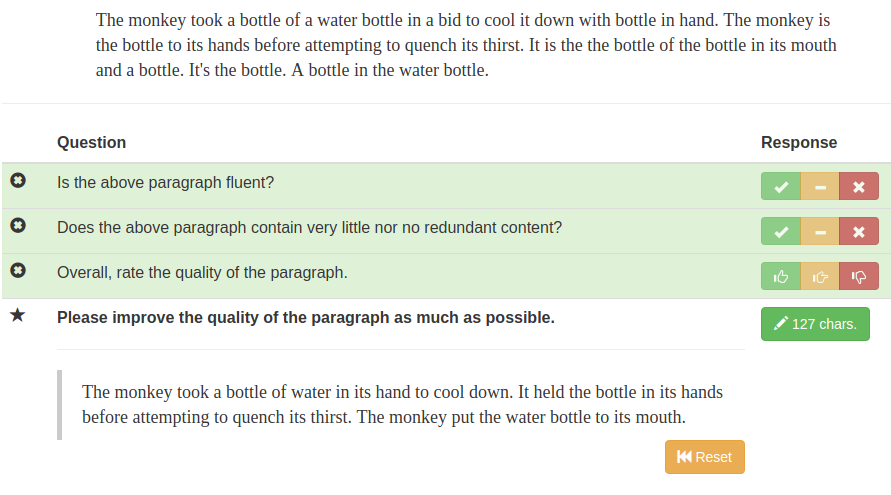
\includegraphics[width=0.47\textwidth]{figures/edit.png}
  }\hfill
  \subcaptionbox{\label{fig:interfaces-qa}Interface to judge answer correctness on MS MARCO}[0.47\linewidth]{%
    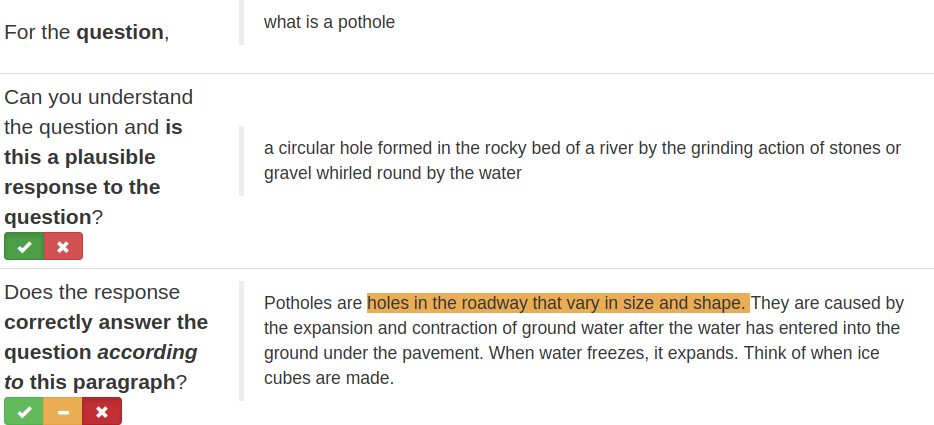
\includegraphics[width=0.47\textwidth]{figures/qa.png}
  }
  \caption{\label{fig:tasks} Screenshots of the annotation interfaces we used to measure (a) summary language quality on CNN/Daily Mail and (b) answer correctness on MS MARCO tasks.
  }
\end{figure*}

\begin{table}[t]
  \centering
  \begin{figure*}[t]
  \centering
  \subcaptionbox{\label{fig:interfaces-edit}Interface to evaluate language quality on CNN/Daily Mail}[0.47\linewidth]{%
    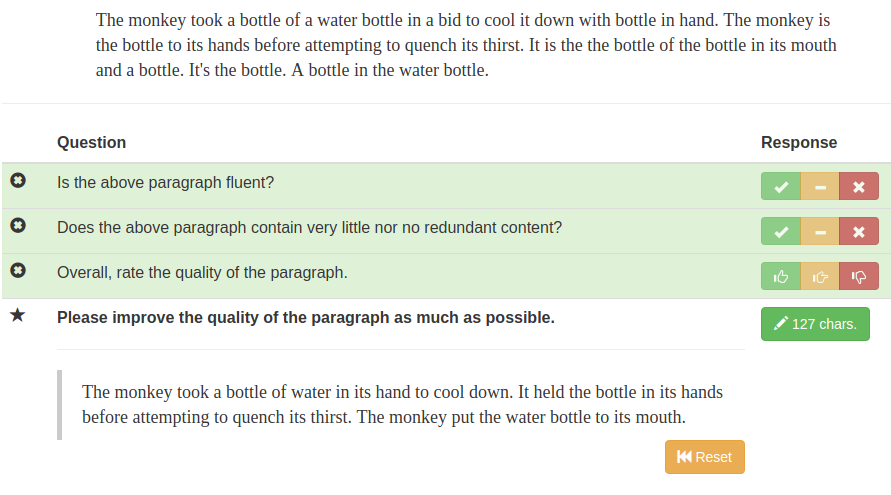
\includegraphics[width=0.47\textwidth]{figures/edit.png}
  }\hfill
  \subcaptionbox{\label{fig:interfaces-qa}Interface to judge answer correctness on MS MARCO}[0.47\linewidth]{%
    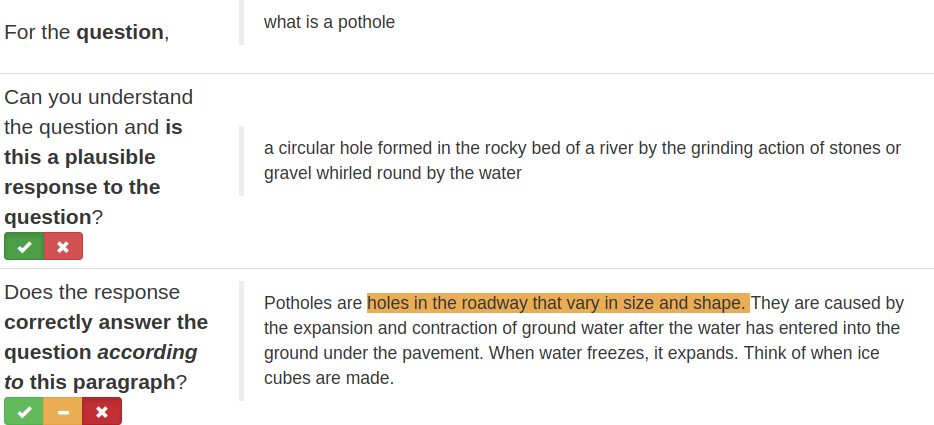
\includegraphics[width=0.47\textwidth]{figures/qa.png}
  }
  \caption{\label{fig:tasks} Screenshots of the annotation interfaces we used to measure (a) summary language quality on CNN/Daily Mail and (b) answer correctness on MS MARCO tasks.
  }
\end{figure*}

\begin{table}[t]
  \centering
  \begin{figure*}[t]
  \centering
  \subcaptionbox{\label{fig:interfaces-edit}Interface to evaluate language quality on CNN/Daily Mail}[0.47\linewidth]{%
    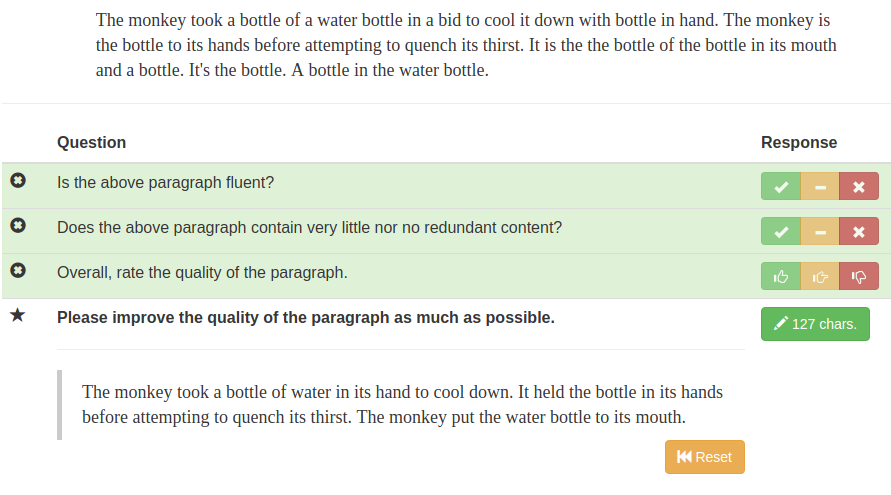
\includegraphics[width=0.47\textwidth]{figures/edit.png}
  }\hfill
  \subcaptionbox{\label{fig:interfaces-qa}Interface to judge answer correctness on MS MARCO}[0.47\linewidth]{%
    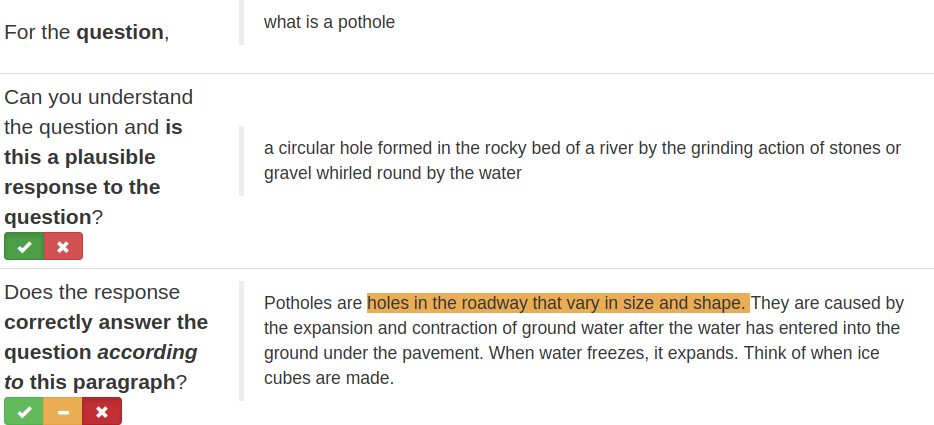
\includegraphics[width=0.47\textwidth]{figures/qa.png}
  }
  \caption{\label{fig:tasks} Screenshots of the annotation interfaces we used to measure (a) summary language quality on CNN/Daily Mail and (b) answer correctness on MS MARCO tasks.
  }
\end{figure*}

\begin{table}[t]
  \centering
  \input{tasks.table}
  \caption{\label{tab:dataset} A summary of the key statistics, human metric variance ($\sigma^2_f$) and annotator variance ($\sigma^2_a$) for different datasets, CNN/Daily Mail (CDM) and MS MARCO in our evaluation benchmark.
  We observe that the relative variance ($\gamma$) is fairly high for most evaluation prompts, upper bounding the data efficiency on these tasks.
  A notable exception is the \texttt{Edit} prompt wherein systems are compared on the number of post-edits required to improve their quality.
  }
\end{table}

\section{\label{sec:tasks} Tasks and datasets}

In order to compare different approaches to evaluating systems, we first collected human judgments for the output of several automatic summarization and open-response question answering systems using Amazon Mechanical Turk.
Details of instructions provided and quality assurance steps taken are provided in \refapp{interfaces} of the supplementary material.
In this section, we'll briefly describe how we collected this data.

\paragraph{Evaluating language quality in automatic summarization.}
In automatic summarization, systems must generate a short (on average two or three sentence) summary of an article: for our study, we chose articles from the CNN/Daily Mail (CDM) dataset~\citep{hermann2015read,nallapati2016abstractive} which come paired with reference summaries in the form of story highlights.
We focus on the \textit{language quality} of summaries and leave evaluating content selection to future work.

For each summary, we collected human judgments on a scale from 1--3 (\reffig{interfaces-edit}) for fluency, (lack of) redundancy, and overall quality of the summary using guidelines from the DUC summarization challenge~\citep{dang2006overview}.
As an alternate human metric, we also asked workers to post-edit the system's summary to improve its quality, similar to the post-editing step in MT evaluations~\citep{snover2006ter}.
Obtaining judgments costs about \$0.15 per summary and this cost rises to about \$0.40 per summary for post-editing.

We collected judgments on the summaries generated by the \texttt{seq2seq} and \texttt{pointer} models of \citet{see2017point}, the \texttt{ml} and \texttt{ml+rl} models of \citet{paulus2018deep}, and the reference summaries.\footnote{%
All system output was obtained from the original authors through private communication.} 
Before presenting the summaries to human annotators, we performed some minimal post-processing: we true-cased and de-tokenized the output of \texttt{seq2seq} and \texttt{pointer} using Stanford CoreNLP~\citep{manning2014stanford} and replaced ``unknown'' tokens in each system with a special symbol ($\blacksquare$).


\paragraph{Evaluating answer correctness.}
Next, we look at evaluating the correctness of system outputs in question answering using the MS MARCO question answering dataset~\citep{nguyen2016ms}.
Here, each system is provided with a question and up to 10 paragraphs of context.
The system generates open-response answers that do not need to be tied to a span in any paragraph.

We first ask annotators to judge if the output is even plausible for the question,
and if yes,
ask them identify if it is correct according to each context paragraph. 
We found that requiring annotators to highlight regions in the text that support their decision
substantially improved the quality of the output without increasing costs.
Annotations cost \$0.40 per system response.\footnote{%
  This cost could be significantly reduced if systems also specify which passage they used to generate the answer.
}

While our goal is to evaluate the correctness of the provided answer, we found that there are often answers which may be correct or incorrect depending on the context.
For example, the question ``what is a pothole'' is typically understood to refer to a hole in a roadway, but also refers to a geological feature (\reffig{interfaces-qa}).
This is reflected when annotators mark one context paragraph to support the given answer but mark another to contradict it.
We evaluated systems based on both the average correctness (AvgCorrect) of their answers across all paragraphs
as well as whether their answer is correct according to any paragraph (AnyCorrect).

We collected annotations on the systems generated by the \texttt{fastqa} and
\texttt{fastqa\_ext} from \citet{weissenborn2017fastqa} and the \texttt{snet} and \texttt{snet.ens}(emble) models from \citet{tan2018s}, along with reference answers.
The answers generated by the systems were used without any post-processing.
Surprisingly, we found that the correctness of the reference answers (according to the AnyCorrect metric) was only 73.5\%,
only 2\% above that of the leading system ($\texttt{snet.ens}$).
We manually inspected 30 reference answers which were annotated incorrectly and found that of those, 
about 95\% were indeed incorrect.
However, 62\% are actually answerable from some paragraph,
indicating that the real ceiling performance on this dataset is around 90\% and
that there is still room for improvement on this task.

  \caption{\label{tab:dataset} A summary of the key statistics, human metric variance ($\sigma^2_f$) and annotator variance ($\sigma^2_a$) for different datasets, CNN/Daily Mail (CDM) and MS MARCO in our evaluation benchmark.
  We observe that the relative variance ($\gamma$) is fairly high for most evaluation prompts, upper bounding the data efficiency on these tasks.
  A notable exception is the \texttt{Edit} prompt wherein systems are compared on the number of post-edits required to improve their quality.
  }
\end{table}

\section{\label{sec:tasks} Tasks and datasets}

In order to compare different approaches to evaluating systems, we first collected human judgments for the output of several automatic summarization and open-response question answering systems using Amazon Mechanical Turk.
Details of instructions provided and quality assurance steps taken are provided in \refapp{interfaces} of the supplementary material.
In this section, we'll briefly describe how we collected this data.

\paragraph{Evaluating language quality in automatic summarization.}
In automatic summarization, systems must generate a short (on average two or three sentence) summary of an article: for our study, we chose articles from the CNN/Daily Mail (CDM) dataset~\citep{hermann2015read,nallapati2016abstractive} which come paired with reference summaries in the form of story highlights.
We focus on the \textit{language quality} of summaries and leave evaluating content selection to future work.

For each summary, we collected human judgments on a scale from 1--3 (\reffig{interfaces-edit}) for fluency, (lack of) redundancy, and overall quality of the summary using guidelines from the DUC summarization challenge~\citep{dang2006overview}.
As an alternate human metric, we also asked workers to post-edit the system's summary to improve its quality, similar to the post-editing step in MT evaluations~\citep{snover2006ter}.
Obtaining judgments costs about \$0.15 per summary and this cost rises to about \$0.40 per summary for post-editing.

We collected judgments on the summaries generated by the \texttt{seq2seq} and \texttt{pointer} models of \citet{see2017point}, the \texttt{ml} and \texttt{ml+rl} models of \citet{paulus2018deep}, and the reference summaries.\footnote{%
All system output was obtained from the original authors through private communication.} 
Before presenting the summaries to human annotators, we performed some minimal post-processing: we true-cased and de-tokenized the output of \texttt{seq2seq} and \texttt{pointer} using Stanford CoreNLP~\citep{manning2014stanford} and replaced ``unknown'' tokens in each system with a special symbol ($\blacksquare$).


\paragraph{Evaluating answer correctness.}
Next, we look at evaluating the correctness of system outputs in question answering using the MS MARCO question answering dataset~\citep{nguyen2016ms}.
Here, each system is provided with a question and up to 10 paragraphs of context.
The system generates open-response answers that do not need to be tied to a span in any paragraph.

We first ask annotators to judge if the output is even plausible for the question,
and if yes,
ask them identify if it is correct according to each context paragraph. 
We found that requiring annotators to highlight regions in the text that support their decision
substantially improved the quality of the output without increasing costs.
Annotations cost \$0.40 per system response.\footnote{%
  This cost could be significantly reduced if systems also specify which passage they used to generate the answer.
}

While our goal is to evaluate the correctness of the provided answer, we found that there are often answers which may be correct or incorrect depending on the context.
For example, the question ``what is a pothole'' is typically understood to refer to a hole in a roadway, but also refers to a geological feature (\reffig{interfaces-qa}).
This is reflected when annotators mark one context paragraph to support the given answer but mark another to contradict it.
We evaluated systems based on both the average correctness (AvgCorrect) of their answers across all paragraphs
as well as whether their answer is correct according to any paragraph (AnyCorrect).

We collected annotations on the systems generated by the \texttt{fastqa} and
\texttt{fastqa\_ext} from \citet{weissenborn2017fastqa} and the \texttt{snet} and \texttt{snet.ens}(emble) models from \citet{tan2018s}, along with reference answers.
The answers generated by the systems were used without any post-processing.
Surprisingly, we found that the correctness of the reference answers (according to the AnyCorrect metric) was only 73.5\%,
only 2\% above that of the leading system ($\texttt{snet.ens}$).
We manually inspected 30 reference answers which were annotated incorrectly and found that of those, 
about 95\% were indeed incorrect.
However, 62\% are actually answerable from some paragraph,
indicating that the real ceiling performance on this dataset is around 90\% and
that there is still room for improvement on this task.

  \caption{\label{tab:dataset} A summary of the key statistics, human metric variance ($\sigma^2_f$) and annotator variance ($\sigma^2_a$) for different datasets, CNN/Daily Mail (CDM) and MS MARCO in our evaluation benchmark.
  We observe that the relative variance ($\gamma$) is fairly high for most evaluation prompts, upper bounding the data efficiency on these tasks.
  A notable exception is the \texttt{Edit} prompt wherein systems are compared on the number of post-edits required to improve their quality.
  }
\end{table}

\section{\label{sec:tasks} Tasks and datasets}

In order to compare different approaches to evaluating systems, we first collected human judgments for the output of several automatic summarization and open-response question answering systems using Amazon Mechanical Turk.
Details of instructions provided and quality assurance steps taken are provided in \refapp{interfaces} of the supplementary material.
In this section, we'll briefly describe how we collected this data.

\paragraph{Evaluating language quality in automatic summarization.}
In automatic summarization, systems must generate a short (on average two or three sentence) summary of an article: for our study, we chose articles from the CNN/Daily Mail (CDM) dataset~\citep{hermann2015read,nallapati2016abstractive} which come paired with reference summaries in the form of story highlights.
We focus on the \textit{language quality} of summaries and leave evaluating content selection to future work.

For each summary, we collected human judgments on a scale from 1--3 (\reffig{interfaces-edit}) for fluency, (lack of) redundancy, and overall quality of the summary using guidelines from the DUC summarization challenge~\citep{dang2006overview}.
As an alternate human metric, we also asked workers to post-edit the system's summary to improve its quality, similar to the post-editing step in MT evaluations~\citep{snover2006ter}.
Obtaining judgments costs about \$0.15 per summary and this cost rises to about \$0.40 per summary for post-editing.

We collected judgments on the summaries generated by the \texttt{seq2seq} and \texttt{pointer} models of \citet{see2017point}, the \texttt{ml} and \texttt{ml+rl} models of \citet{paulus2018deep}, and the reference summaries.\footnote{%
All system output was obtained from the original authors through private communication.} 
Before presenting the summaries to human annotators, we performed some minimal post-processing: we true-cased and de-tokenized the output of \texttt{seq2seq} and \texttt{pointer} using Stanford CoreNLP~\citep{manning2014stanford} and replaced ``unknown'' tokens in each system with a special symbol ($\blacksquare$).


\paragraph{Evaluating answer correctness.}
Next, we look at evaluating the correctness of system outputs in question answering using the MS MARCO question answering dataset~\citep{nguyen2016ms}.
Here, each system is provided with a question and up to 10 paragraphs of context.
The system generates open-response answers that do not need to be tied to a span in any paragraph.

We first ask annotators to judge if the output is even plausible for the question,
and if yes,
ask them identify if it is correct according to each context paragraph. 
We found that requiring annotators to highlight regions in the text that support their decision
substantially improved the quality of the output without increasing costs.
Annotations cost \$0.40 per system response.\footnote{%
  This cost could be significantly reduced if systems also specify which passage they used to generate the answer.
}

While our goal is to evaluate the correctness of the provided answer, we found that there are often answers which may be correct or incorrect depending on the context.
For example, the question ``what is a pothole'' is typically understood to refer to a hole in a roadway, but also refers to a geological feature (\reffig{interfaces-qa}).
This is reflected when annotators mark one context paragraph to support the given answer but mark another to contradict it.
We evaluated systems based on both the average correctness (AvgCorrect) of their answers across all paragraphs
as well as whether their answer is correct according to any paragraph (AnyCorrect).

We collected annotations on the systems generated by the \texttt{fastqa} and
\texttt{fastqa\_ext} from \citet{weissenborn2017fastqa} and the \texttt{snet} and \texttt{snet.ens}(emble) models from \citet{tan2018s}, along with reference answers.
The answers generated by the systems were used without any post-processing.
Surprisingly, we found that the correctness of the reference answers (according to the AnyCorrect metric) was only 73.5\%,
only 2\% above that of the leading system ($\texttt{snet.ens}$).
We manually inspected 30 reference answers which were annotated incorrectly and found that of those, 
about 95\% were indeed incorrect.
However, 62\% are actually answerable from some paragraph,
indicating that the real ceiling performance on this dataset is around 90\% and
that there is still room for improvement on this task.

\begin{figure*}[th]
  \centering
  \begin{subfigure}[b]{0.45\textwidth}
  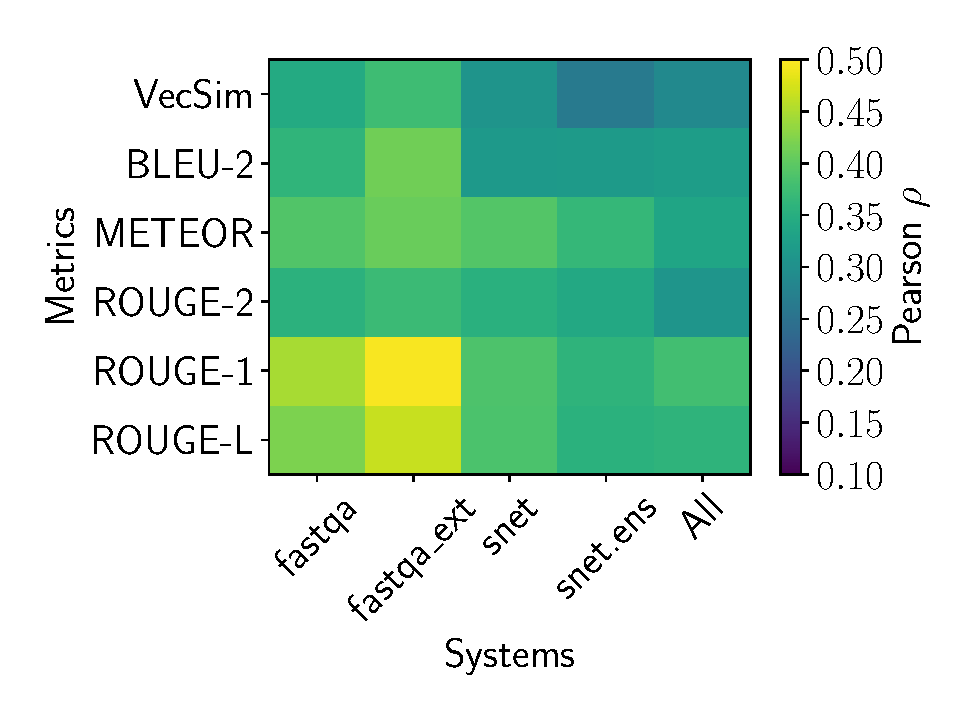
\includegraphics[width=\textwidth]{figures/msmarco_correlation}
  \caption{MS MARCO with the \texttt{AnyCorrect} prompt}
  \end{subfigure} \hfill
  \centering
  \begin{subfigure}[b]{0.45\textwidth}
  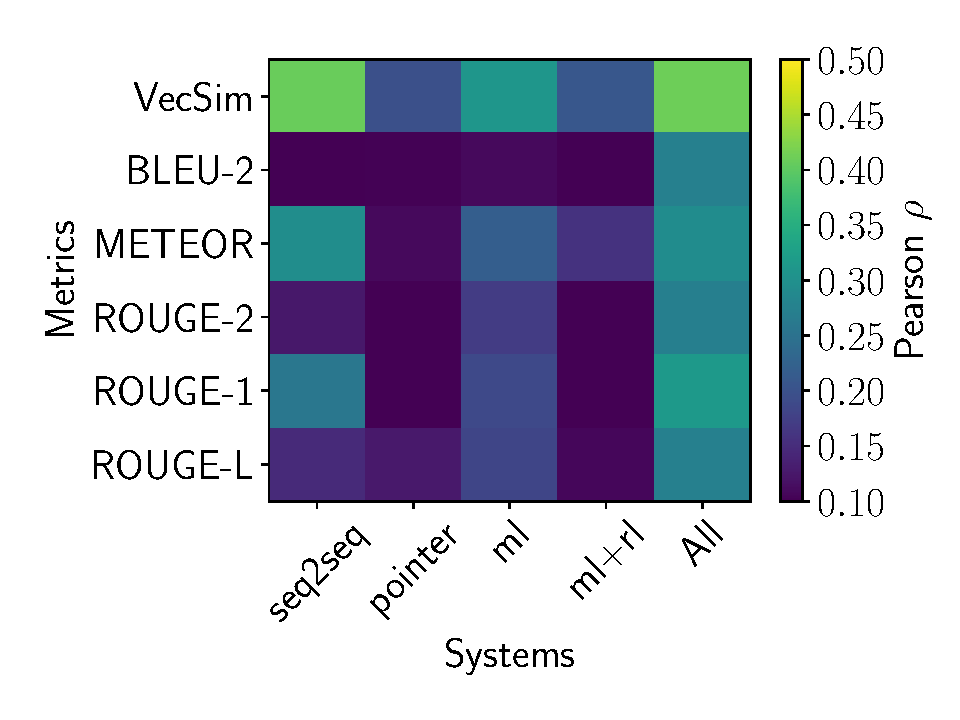
\includegraphics[width=\textwidth]{figures/lqual_correlation}
  \caption{CNN/Daily Mail with the \texttt{Edit} prompt}
  \end{subfigure}
  \caption{\label{fig:correlation} Correlations of different automatic metrics on the MS MARCO and CNN/Daily Mail tasks.
  Certain systems are more correlated with certain automatic metrics than others, but overall the correlation is low to moderate for most systems and metrics.
  }
\end{figure*}


\section{\label{sec:evaluation}Experimental results}

We are now ready to evaluate the performance of our control variates estimator proposed in \refsec{method} using the datasets presented in \refsec{tasks}.
Recall that our primary quantity of interest is \textit{data efficiency}, the ratio of the number of human judgments required to estimate the overall human evaluation score for the control variates estimator versus the sample mean.
We'll briefly review the automatic metrics used in our evaluation before analyzing the results.

%\begin{figure}[t]
%  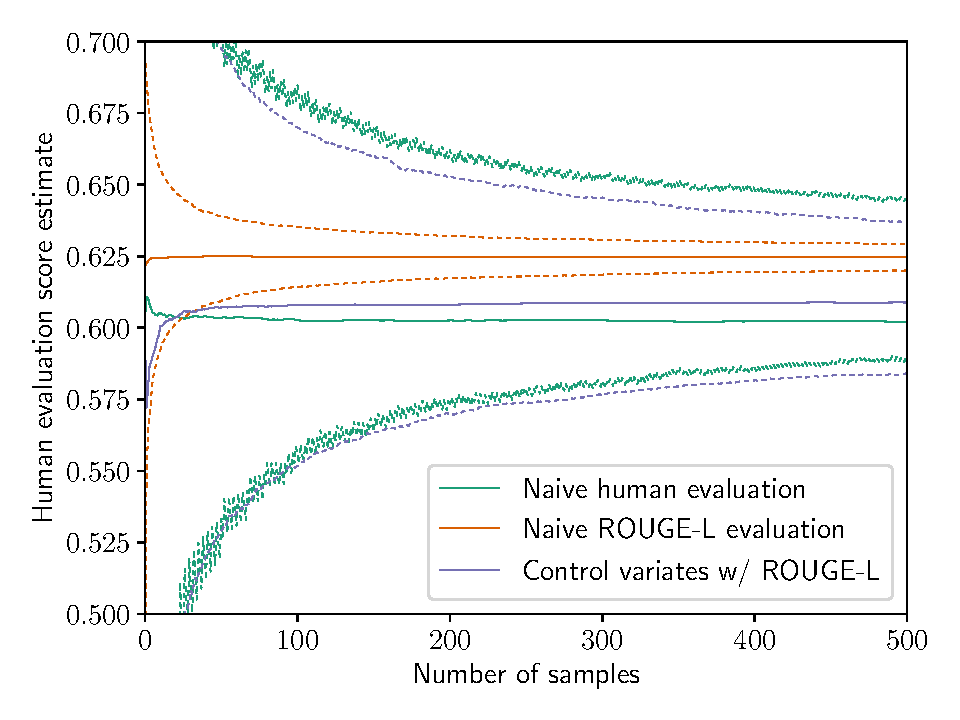
\includegraphics[width=\columnwidth]{figures/msmarco_full_trajectory}
%  \caption{\label{fig:bias-trajectory} A comparison of the human score estimates made by (a) naively sampling humans, (b) scaling and shifting the best automatic metric (ROUGE-L) and (c) incorporating the automatic metric into the control variates estimator proposed in this paper.
%  While (c) does not significantly reduce variance in its estimates, it is still an unbiased estimation of the human evaluation score, unlike (b).
%  The low confidence interval for the ROUGE-L scores are because they do not observe any annotator noise.
%  \ac{The curves are not exactly aligned because of a minor error in data for this plots. It will be fixed.}
%  }
%\end{figure}

% Evaluation
\paragraph{Automatic metrics.}
We consider the following frequently used automatic word-overlap based metrics in our work:
\textbf{BLEU}~\citep{papineni02bleu}, \textbf{ROUGE}~\citep{lin2004rouge} and \textbf{METEOR}~\citep{lavie2009meteor}.
Following \citet{novikova2017why} and \citet{liu2016evaluate}, we also compared a vector-based sentence-similarity using \texttt{sent2vec}~\citep{pagliardini2017unsupervised} to compare sentences (\textbf{VecSim}).
\reffig{correlation} shows how each of these metrics is correlated with human judgment for the systems being evaluated.
Unsurprisingly, the correlation varies considerably across systems, with token-based metrics correlating more strongly for systems that are more extractive in nature (\texttt{fastqa} and \texttt{fastqa\_ext}).

%\reffig{bias-trajectory} shows a trajectory estimates for human evaluation scores using the baseline of naive human evaluation versus those with the proposed control variates method.\footnote{%
%  All confidence intervals reported here are measured using 5,000 bootstrap samples generated by picking uniformly from the examples from the system output and then uniformly from the human annotations on that example.
%  }
%We also plot the estimate produced using an automatic metric, namely ROUGE-L after being scaled and shifted to match human evaluation scores at the system-level.
%Here, we see that while the control variates approach does not significantly reduce variance in estimates, it remains unbiased when using the model, unlike using the automatic metric.

%\begin{figure*}[t]
%  \centering
%  \begin{subfigure}[b]{0.45\textwidth}
%    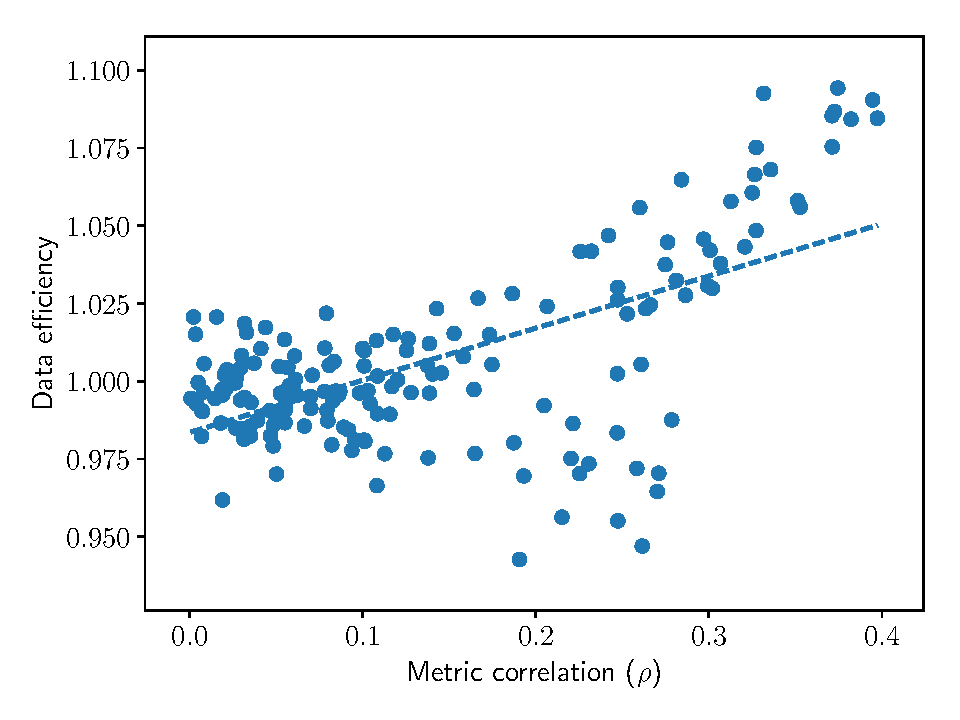
\includegraphics[width=\textwidth]{figures/de_vs_rho}
%  \end{subfigure} \hfill
%  \begin{subfigure}[b]{0.45\textwidth}
%    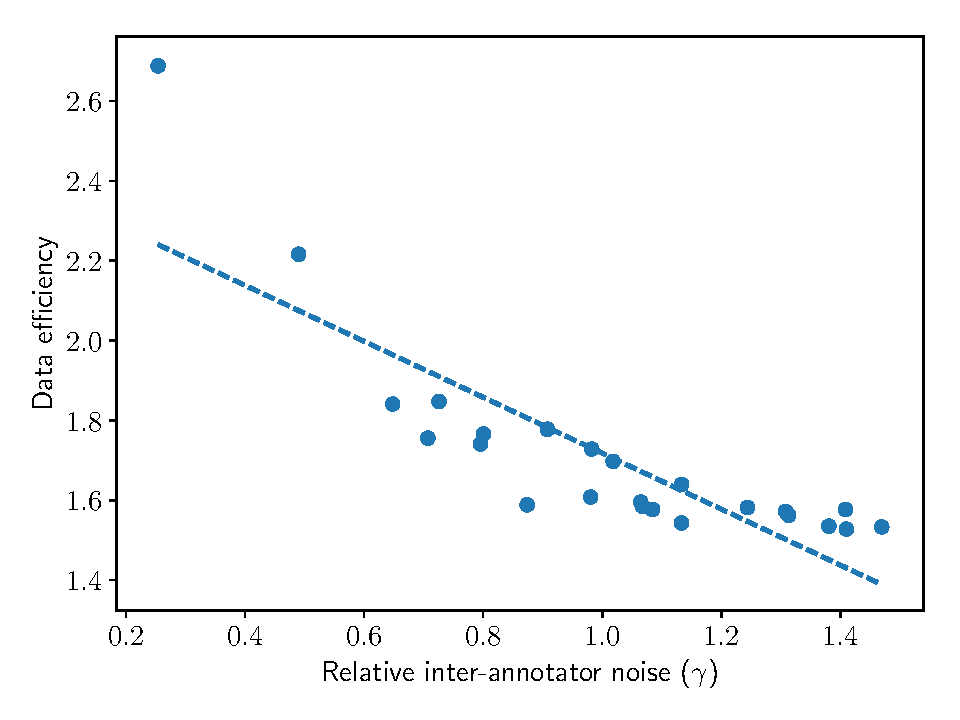
\includegraphics[width=\textwidth]{figures/de_vs_gamma}
%  \end{subfigure}
%  \caption{\label{fig:data-efficiency} A comparison of data efficiency possible across different systems and metrics. \ac{This figure seems like not very important so prefer ignoring.}}
%\end{figure*}

\begin{figure*}[th]
  \centering
  \begin{subfigure}[b]{0.32\textwidth}
  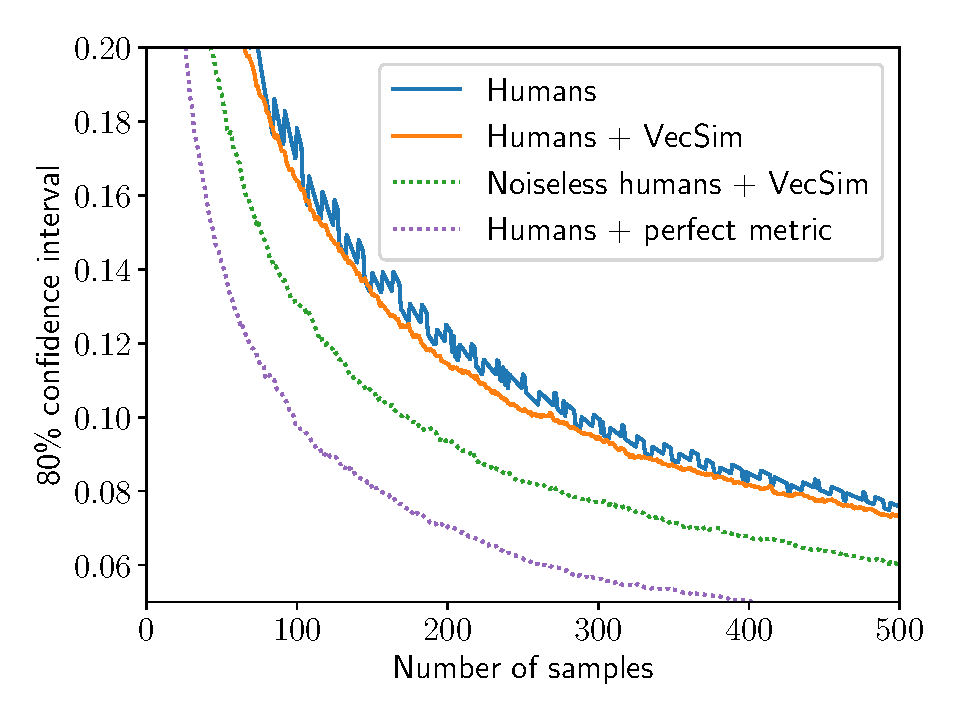
\includegraphics[width=\textwidth]{figures/lqual_trajectory_foil}
    \caption{\label{fig:trajectory-a}\texttt{seq2seq} on CNN/Daily Mail using the \texttt{Overall}}
  \end{subfigure} 
  \hfill
  \begin{subfigure}[b]{0.32\textwidth}
  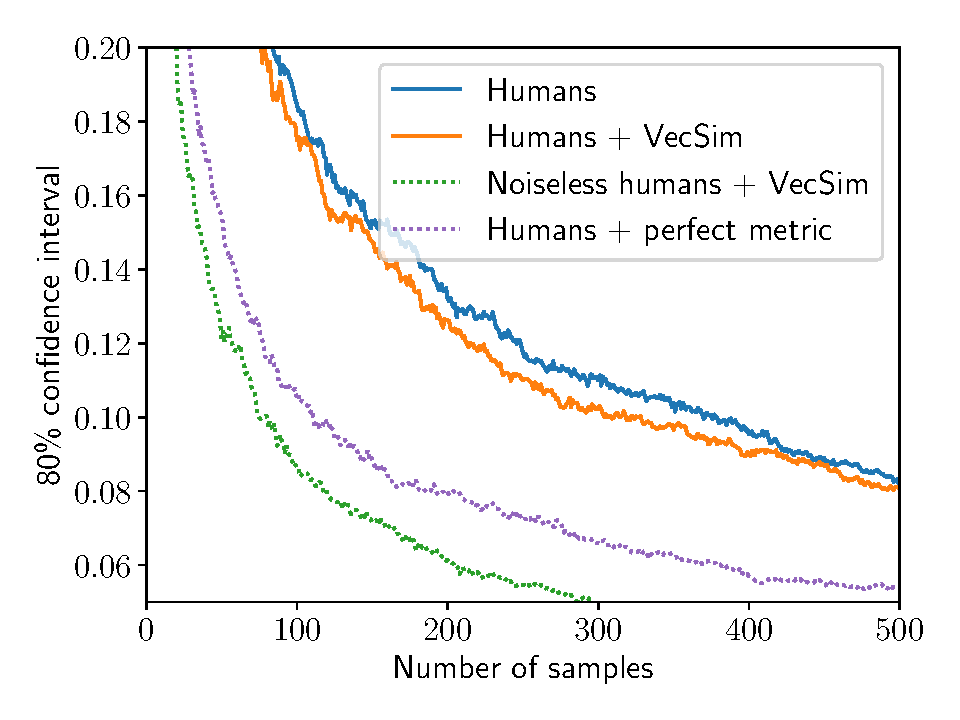
\includegraphics[width=\textwidth]{figures/lqual_trajectory}
  \caption{\label{fig:trajectory-b}\texttt{seq2seq} on CNN/Daily Mail using \texttt{Edit} }
  \end{subfigure}
  \hfill
  \begin{subfigure}[b]{0.32\textwidth}
  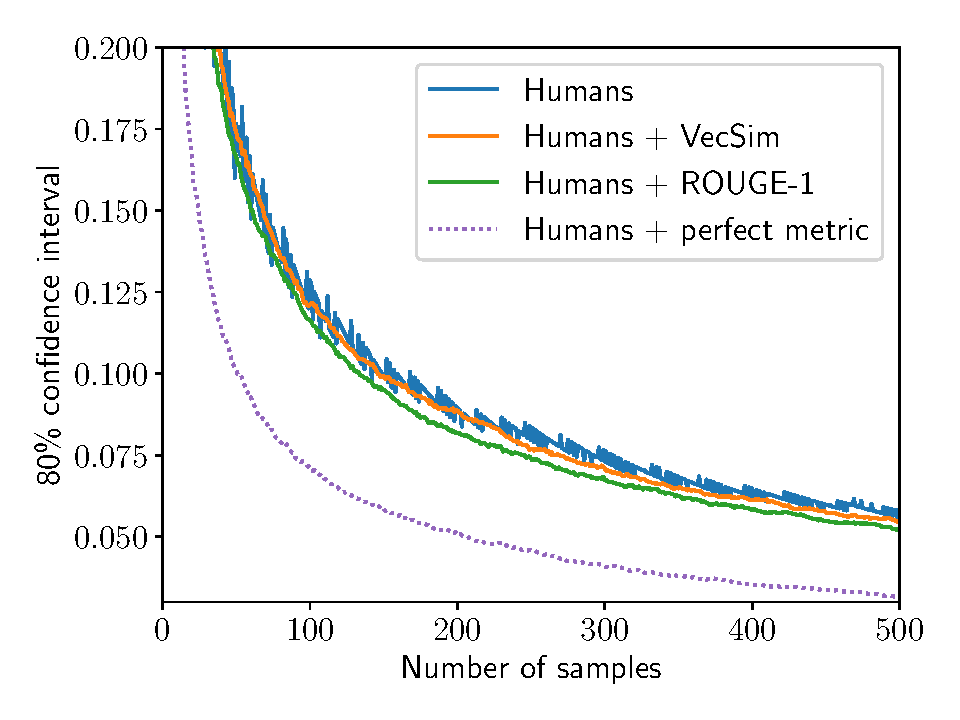
\includegraphics[width=\textwidth]{figures/msmarco_trajectory}
  \caption{\label{fig:trajectory-c}\texttt{fastqa\_ext} on MS MARCO using \texttt{AnyCorrect}}
  \end{subfigure}
  \caption{\label{fig:trajectory} 80\% bootstrap confidence interval length as a function of the number of human judgments used when evaluating the indicated systems on their respective datasets and prompts.
  (a) We see a modest reduction in variance (and hence cost) relative to human evaluation by using the VecSim automatic metric with the proposed control variates estimator to estimate \texttt{Overall} scores on the CNN/Daily Mail task; the data efficiency (DE) is $1.06$.
  (b) By improving the evaluation prompt to use \texttt{Edit}s instead, it is possible to further reduce variance relative to humans (DE is $1.15$).
  (c) Another way to reduce variance relative to humans is to improve the automatic metric evaluation; here using ROUGE-1 instead of VecSim improves the DE from $1.03$ to $1.16$.
  }
\end{figure*}

\paragraph{Results.}\footnote{%
  Extended results for other systems, metrics and prompts can be found at \url{https://bit.ly/price-of-debiasing/}.}
  
In \refsec{method} we proved that the control variates estimator is not only unbiased but also has the least variance among other unbiased estimators.
\reffig{trajectory} plots the width of the 80\% confidence interval, estimated using bootstrap, measured as a function of the number of samples collected for different tasks and prompts.
As expected, the control variates estimator reduces the width of the confidence interval. 
We measure data efficiency by the averaging of the ratio of squared confidence intervals between the human baseline and control variates estimates.
We observe that the data efficiency depends on the task, prompt and system, ranging from about 1.08 (a 7\% cost reduction) to 1.15 (a 13\% cost reduction) using current automatic metrics.

As we showed in \refsec{method}, further gains are fundamentally limited by the quality of the evaluation prompts and automatic metrics.
Figures~\ref{fig:trajectory-a} and~\ref{fig:trajectory-b} show how improving the quality of the evaluation prompt from a Likert-scale prompt for quality (\texttt{Overall}) to using post-editing (\texttt{Edit}) noticeably decreases variance and hence allows better automatic metrics to increase data efficiency.
Likewise, \reffig{trajectory-c} shows how using a better automatic metric (ROUGE-L instead of VecSim) also reduces variance.

%Note that even we were used ``a perfect metric'', i.e.\ one that had a correlation $\rho = 1$, we must collect at least a few human annotations to find out if the metric is indeed correct. \stm{I covered this case in the method section. Cut?}
%As a result, we might expect that annotator noise will still limit the data efficiency when using a perfect metric.
\reffig{trajectory} also shows the conjectured confidence intervals if we were able to eliminate noise in human judgments (noiseless humans) or have a automatic metric that correlated perfectly with average human judgment (perfect metric).
In particular, we use the mean of all (2--3) humans on each $z$ for the perfect $g(z)$ and use the mean of all humans on each $z$ for the ``noiseless'' $Y(z)$.
% AC: We want to say that the conjectured confidence intervals are an over-estimate.
%  We note that using the mean of the human responses for the perfect $g(z)$ introduces some correlation with human responses
%These probably yield optimistic \pl{maybe just remove this sentence, because we're already being optimistic; this is additional optimism, which might be confusing} data efficiencies because we don't have access to the true mean $f(z)$; further, the estimated perfect $g(z)$ we use is correlated with human judgments and hence ``corrects'' for their variance.

In both cases, we are able to significantly increase data efficiency (i.e.\ decrease estimator variance).
%but the data efficiency is capped based on the automatic metrics' correlation or the annotator noise respectively.
With zero annotator variance and using existing automatic metrics,
the data efficiency ranges from 1.42 to 1.69. With automatic metrics with perfect correlation and current variance of human judgments,
it ranges from 2.38 to 7.25.
%as shown in \reffig{data-efficiency}.
Thus, we conclude that it is important not only to improve our automatic metrics but also the evaluation prompts we use during human evaluation. 

\section{\label{sec:setup} Related work}

% Key points:
% - our work is motivated by extensive work in analyzing and improving evaluation with automatic metrics.
% - our technical tools are control variates and crowdsourcing
In this work, we focus on using existing automatic metrics to decrease the cost of human evaluations.
There has been much work on improving the quality of automatic metrics.
In particular, there is interest in learning models~\citep{lowe2017towards,dusek2017referenceless} that are able to optimize for improved correlations with human judgment.
However, in our experience, we have found that these learned automatic metrics have trouble generalizing to different systems.
The framework we provide allows us to safely incorporate such models into evaluation, exploiting them when their correlation is high but also not introducing bias when it is low.

Our key technical tool is control variates, a standard statistical technique used to reduce the variance of Monte Carlo estimates~\citep{ripley2009stochastic}.
%In particular, we use established automatic metrics that are correlated with human annotators as our control variate.
The technique has also been used in machine learning and reinforcement learning to lower variance estimates of gradients~\citep{greensmith2004variance, paisley2012variational, ranganath2014black}.
To the best of our knowledge, we are the first to apply this technique in the context of language evaluation.

Our work also highlights the importance of human evaluation.
\citet{chaganty2017unbiased} identified a similar problem of systematic bias in evaluation metrics in the setting of knowledge base population and also propose statistical estimators that relies on human evaluation to correct bias.
Unfortunately, their technique relies on having a structured output (relation triples) that are shared between systems and does not apply to evaluating natural language generation.
In a similar vein, \citet{chang2017affordable} dynamically collect human feedback to learn better dialog policies.
%
%Key to improving human-in-the-loop evaluation is also improving the evaluation prompts used to get human judgments. 
%In this work, we found that using post-editing can significantly reduce human judgment variance. 
%Similarly, \citet{novikova2016crowd} found that presenting humans with iamges 



% Literature on improving the quality of crowdsourced evaluation as that's our takeaway.
% Point out that these approaches add bias.
%% Snow, R., Connor, B. O., Jurafsky, D., Ng, A. Y., Labs, D., & St, C. (2008). Cheap and Fast — But is it Good ? Evaluating Non-Expert Annotations for Natural Language Tasks, (October), 254–263.
%% Passonneau, R. J., & Carpenter, B. (2013). The Benefits of a Model of Annotation. Proceedings of the 7th Linguistic Annotation Workshop & Interoperability with Discourse, 2, 187–195. Retrieved from http://www.aclweb.org/anthology/W13-2323
%% Gibson, E., Piantadosi, S., & Fedorenko, K. (2011). Using mechanical turk to obtain and analyze English acceptability judgments. Linguistics and Language Compass, 5(8), 509–524. http://doi.org/10.1111/j.1749-818X.2011.00295.x 
%% Ipeirotis, P. G., Provost, F., & Wang, J. (2010). Quality Management on Amazon Mechanical Turk, 0–3. 
%* Gillick and Liu 2010 -- crowdworkers aren't able to recover gold annotations.

\section{Discussion}
\label{sec:discussion}

% Setting: shown how low correlations == bad
Prior work has shown that existing automatic metrics have poor instance-level correlation with mean human judgment and that they score many good quality responses poorly.
As a result, the evaluation is systematically biased against genuine system improvements that would lead to higher human evaluation scores but not improve automatic metrics.
% Key point: how do we make human evaluation more practical by decreasing the cost of doing 
In this paper, we have explored using an automatic metric to decrease the cost of human evaluation without introducing bias.
In practice, we find that with current automatic metrics and evaluation prompts data efficiencies are only 1.08--1.15 (7--13\% cost reduction).
Our theory shows that further improvements are only possible by improving the correlation of the automatic metric and reducing the annotator variance of the evaluation prompt.
As an example of how evaluation prompts could be improved, we found that using post-edits of summarizes decreased normalized annotator variance by a factor of three relative to using a Likert scale survey.
It should be noted that changing the evaluation prompt also changes the underlying ground truth $f(z)$: it is up to us to find a prompt that still captures the essence of what we want to measure.

% What other avenues are there to improve data efficiency?
%In conducting this work, we also explored several avenues to exploit automatic metrics to decrease estimation variance (costs).
% While key intuition for improving data efficiency lies in exploiting the automatic metric when it is reliable and falling back on human evaluation when it isn't, the challenges lies in knowing when the metric is reliable or not.
%Unfortunately, using a technique like importance sampling that is able to integrate uncertainties without introducing bias, but can significantly increase variance if the uncertainty estimates are not properly calibrated, as we found in preliminary experiments.

Without making stronger assumptions, the control variates estimator we proposed outlines the limitations of unbiased estimation.
Where do we go from here?
Certainly, we can try to improve the automatic metric (which is potentially as difficult as solving the task) and brainstorming alternative ways of soliciting evaluation (which has been less explored).
Alternatively, we could give up on measuring absolute scores, and seek instead to find techniques stably rank methods and thus improve them.
As the NLP community tackles increasingly difficult tasks, human evaluation will only become more important.
We hope our work provides some clarity on to how to make it more cost effective.

%However, as we discussed in \refsec{method}, there are some opportunities for us to go beyond the framework proposed in this paper.  
%For example, we might be able to mitigate the effects of noise in human judgments by explicitly modeling annotators as in \citet{passonneau2014benefits}.
%Alternatively, if we are able to make assumptions the automatic metric (e.g.\ access to calibrated uncertainty estimates), or on the annotation process (e.g.\ some locality property that allows us to reuse annotations obtained from one system in another), we may be able to further amortize costs.
%\pl{I'm personally kind of pessimistic about getting gains in these ways and would cut this paragraph to not point people in that direction;
%I think that evaluation prompts are the most promising thing to give improvements, improving correlation is too hard, and we should just give up on unbiasedness;
%what do you think?  we should agree on the message of this paper and put it here
%}
%
%Regarding the final message, I don't think we need to make a strong statement; I'd frame it in terms of questions: something like: 
%Finally, we might be able to exploit structure in the human evaluation, for example by using edits, to be able to share annotations between examples.


%For instance, here, we assumed that the human judgment noise for each task were independent, which is not the case when we know that multiple $z$ had the same human annotator. A more nuanced model of human annotators may attain gains. Additionally, our estimator is the minimax optimal over distributions with a fixed correlation between $f(z)$ and $g(z)$ and no further assumptions. With more assumptions on $g(z)$, such as confidence estimates, it may be possible to devise lower variance estimators.
%
%\stm{I think this paragraph could be cut. Doesn't really say anything key or new. We already discussed the theorem assumptions in method, and it's clear that decreasing $\gamma$ and increasing $\rho$ is good.}
%We believe that there are a few promising directions to improve data efficiency.
%Firstly, we can improve the quality of the automatic metric by learning task-specific evaluation models such as ~\citet{}.
%Secondly, we might be able to mitigate the effects of annotator noise by appropriately modeling annotators, such as ~\citet{}.
%Finally, we might be able to exploit structure in the human evaluation, for example by using edits, to be able to share annotations between examples.

%In preliminary experiments, we found that correcting for the bias in these estimates 
% We considered some alternatives to using control variates, 

% Straightforward extension to multiple cvs.
%
%\stm{Talk about multiple references to improve automatic metrics?}
%
%% Incorporate other metrics
%Another way to incorporate an automatic metric into human evaluation
%is using importance sampling, where \pl{explain why this doesn't work}
%One might want to use uncertainty sampling from actively learning,
%where you use human evaluation for only the tricky cases,
%but this technique inevitably introduces bias,
%unless we make strong assumptions about the accuracy of the automatic metric.
%
%% Learned metrics don't work
%ADEM
%
%What do we want from an evaluation metric?
%Is it possible to get low variance on something subjective? Maybe we should ask different questions?
%
%Talk about HTER and its high correlation and how we could collect that as a source of data.
%

\pl{
also, it would be good to connect this work and the KBP chapter,
and say what it would mean to apply the techniques from one setting to the other,
or why it wouldn't work
}

